\chapter{Entwurf Missionsplaner}

\section{Geforderte Funktionen}

Die geforderten Funktionen können in fünf Kategorien eingeteilt werden.
\renewcommand{\labelenumi}{\roman{enumi}}
\begin{enumerate}
\item 	Scout-Modus mit Parklückensuche
\item 	Einparken
\item	Parken
\item	Ausparken
\item	Inaktiv sein
\end{enumerate}

\noindent Diese Kategorien definieren die Hauptzustände.\\

\noindent Was das Fahrzeug in jener Kategorie machen soll, ist in den Unterzuständen definiert.\\


\noindent Scout-Modus bedeutet, dass das Fahrzeug einen Parcours abfährt. Dabei wird einer Linie gefolgt. Wenn eine Ecke detektiert wird, muss die Geschwindigkeit reduziert werden. Das Ziel dabei ist, dass die Regelung genauer arbeiten kann und die Kurve abgefahren wird. Während dem Abfahren sucht der Roboter nach Parklücken.\\

\noindent In dem Zustand \glqq Park\_This\grqq{} wird als erstes die Startpose angefahren. Danach wird ein Polynom abgefahren. Wenn die Zielpose in der Lücke erreicht ist, wechselt der Automat automatisch in den Zustand \glqq Park\grqq{}. In diesem wird gewartet, bis über die App das Ausparksignal übermittelt wird.\\

\noindent Beim Ausparken folgt der Roboter erneut einem Polynom zurück auf die Linie. Dabei muss sichergestellt werden, dass nach vorne genügen Freiraum vorhanden ist, sonst gibt es einen Unfall mit der Bande.\\

\noindent Vor allem für das Ein - und Ausparken müssen neben den Hauptzuständen die jeweiligen Unterzustände abgespeichert werden, damit beim Fortsetzen die richtigen Aktionen ausgeführt werden. Bei den Abfahrtspolynomen muss beachtet werden, dass kein neues Polynom berechnet wird. 



\section{Hauptzustandsmaschine}

Für den Entwurf der folgenden Zustandsmaschinen wurde sich an den geforderten Funktionen orientiert. Dabei wurde beachtet, dass die Aufteilung so getätigt wird, dass die Zustandsübergange möglichst einfach sind.\\

\noindent \begin{tabular}{|p{1.5cm}|p{4cm}|p{3.8cm}|p{3cm}|}
	\hline 
	Zustand & Eingangsaktion & Nominalaktion & Ausgangsaktion \\ 
	\hline 
	Driving & Auswahl des Controlmodus & siehe Unterzustandsmaschine & Parklückensuche ausschalten \\ 
	\hline 
	 & Parklückensuche einschalten (Ausnahme bei der Anfahrt) &  &  \\ 
	\hline
	Inactive & Setzen des Controlmodus \glqq INACTIVE\grqq{} & siehe Unterzustandsmaschine &  \\ 
	\hline 
	& Abspeichern des Vorzustandes & &  \\ 
	\hline 
	Exit &  & Abschalten des Systems &  \\ 
	\hline
	Park & Auswahl Controlmodus \glqq INACTIVE\grqq & Ausgabe Sensordaten (Abstand nach vorn und hinten, Position) &  \\ 
	\hline
	Park This & Auswahl des richtigen Subzustandes & siehe Unterzustandsmaschine &  \\ 
	\hline
	 & Parkplatzinformation abfragen &  &  \\ 
	\hline
	 & Variable \glqq anfahrt\grqq und \glqq correct\grqq auf falsch setzen &  &  \\
	\hline
	Park Out & Auswahl des richtigen Subzustands & siehe Unterzustandsmaschine &  \\ 
	\hline 
	 & 	Variable \glqq back\grqq & & \\
	\hline
\end{tabular} 

\begin{figure}[h]
	\centering
	\includegraphics[width=0.9\textwidth]{Zustandsautomataußen}
	\caption{Entwurf Hauptzustandsautomat}
	\label{img:grafik-Hauptzustandsautomat}
\end{figure}

\section{Unterzustandsmaschine}

\subsection{Scout-Modus}

\begin{tabular}{|p{1.5cm}|p{4cm}|p{4cm}|p{3cm}|}
	\hline 
	Zustand & Eingangsaktion & Nominalaktion & Ausgangsaktion \\ 
	\hline 
	Slow & Controlmodusauswahl \glqq SLOW\grqq  &  &  \\ 
	\hline 
	Fast & Controlmodusauswahl \glqq FAST\grqq  &  &  \\ 
	\hline 
\end{tabular} 

\subsection{Pause}

Es gibt keine Unterzustandsmaschine.

\subsection{Exit}

Es gibt keine Unterzustandsmaschine.

\subsection{Park}

Es gibt keine Unterzustandsmaschine.

\subsection{Park This}

\begin{tabular}{|p{1.5cm}|p{4cm}|p{4cm}|p{3cm}|}
	\hline 
	Zustand & Eingangsaktion & Nominalaktion & Ausgangsaktion \\ 
	\hline 
	To Slot & Zielwinkelberechnung & Zustand \glqq DRIVING\grqq bis Pose erreicht ist &  \\ 
	\hline 
	 & Anfahrort festlegen &  &  \\ 
	\hline
	Reached Slot & Start- und Endpose vom Polynom festlegen &  &  \\ 
	\hline
	 & Geschwindigkeit festlegen &  &  \\ 
	\hline 
	 & Setzen des Controlmodus \glqq PARK\_CTRL\grqq   & Überprüfung ob Polynom abgefahren wurde &  \\ 
	\hline
	In Slot &  & Variable \glqq back\grqq  auf wahr setzen &  \\ 
	\hline 
	
\end{tabular} 

\subsection{Park Out}

\begin{tabular}{|p{1.7cm}|p{4cm}|p{4cm}|p{3cm}|}
	\hline 
	Zustand & Eingangsaktion & Nominalaktion & Ausgangsaktion \\ 
	\hline 
	Backwarts & Berechnung der Rückfahrdistanz & Überprüfung ob das Zurückfahren erfolgt ist &  \\ 
	\hline
	 & Setzen des Controlmodus \glqq SETPOSE\grqq & &\\ 
	\hline
	ParkOut & Start- und Endpose vom Polynom festlegen  & Überprüfung ob Polynom abgefahren wurde  &  \\ 
	\hline 
	 & Geschwindigkeit festlegen  &  &  \\ 
	\hline  
	& Setzen des Controlmodus \glqq PARK\_CTRL\grqq & &  \\ 
	\hline
 
\end{tabular} 

\begin{figure}[h]
	\centering
	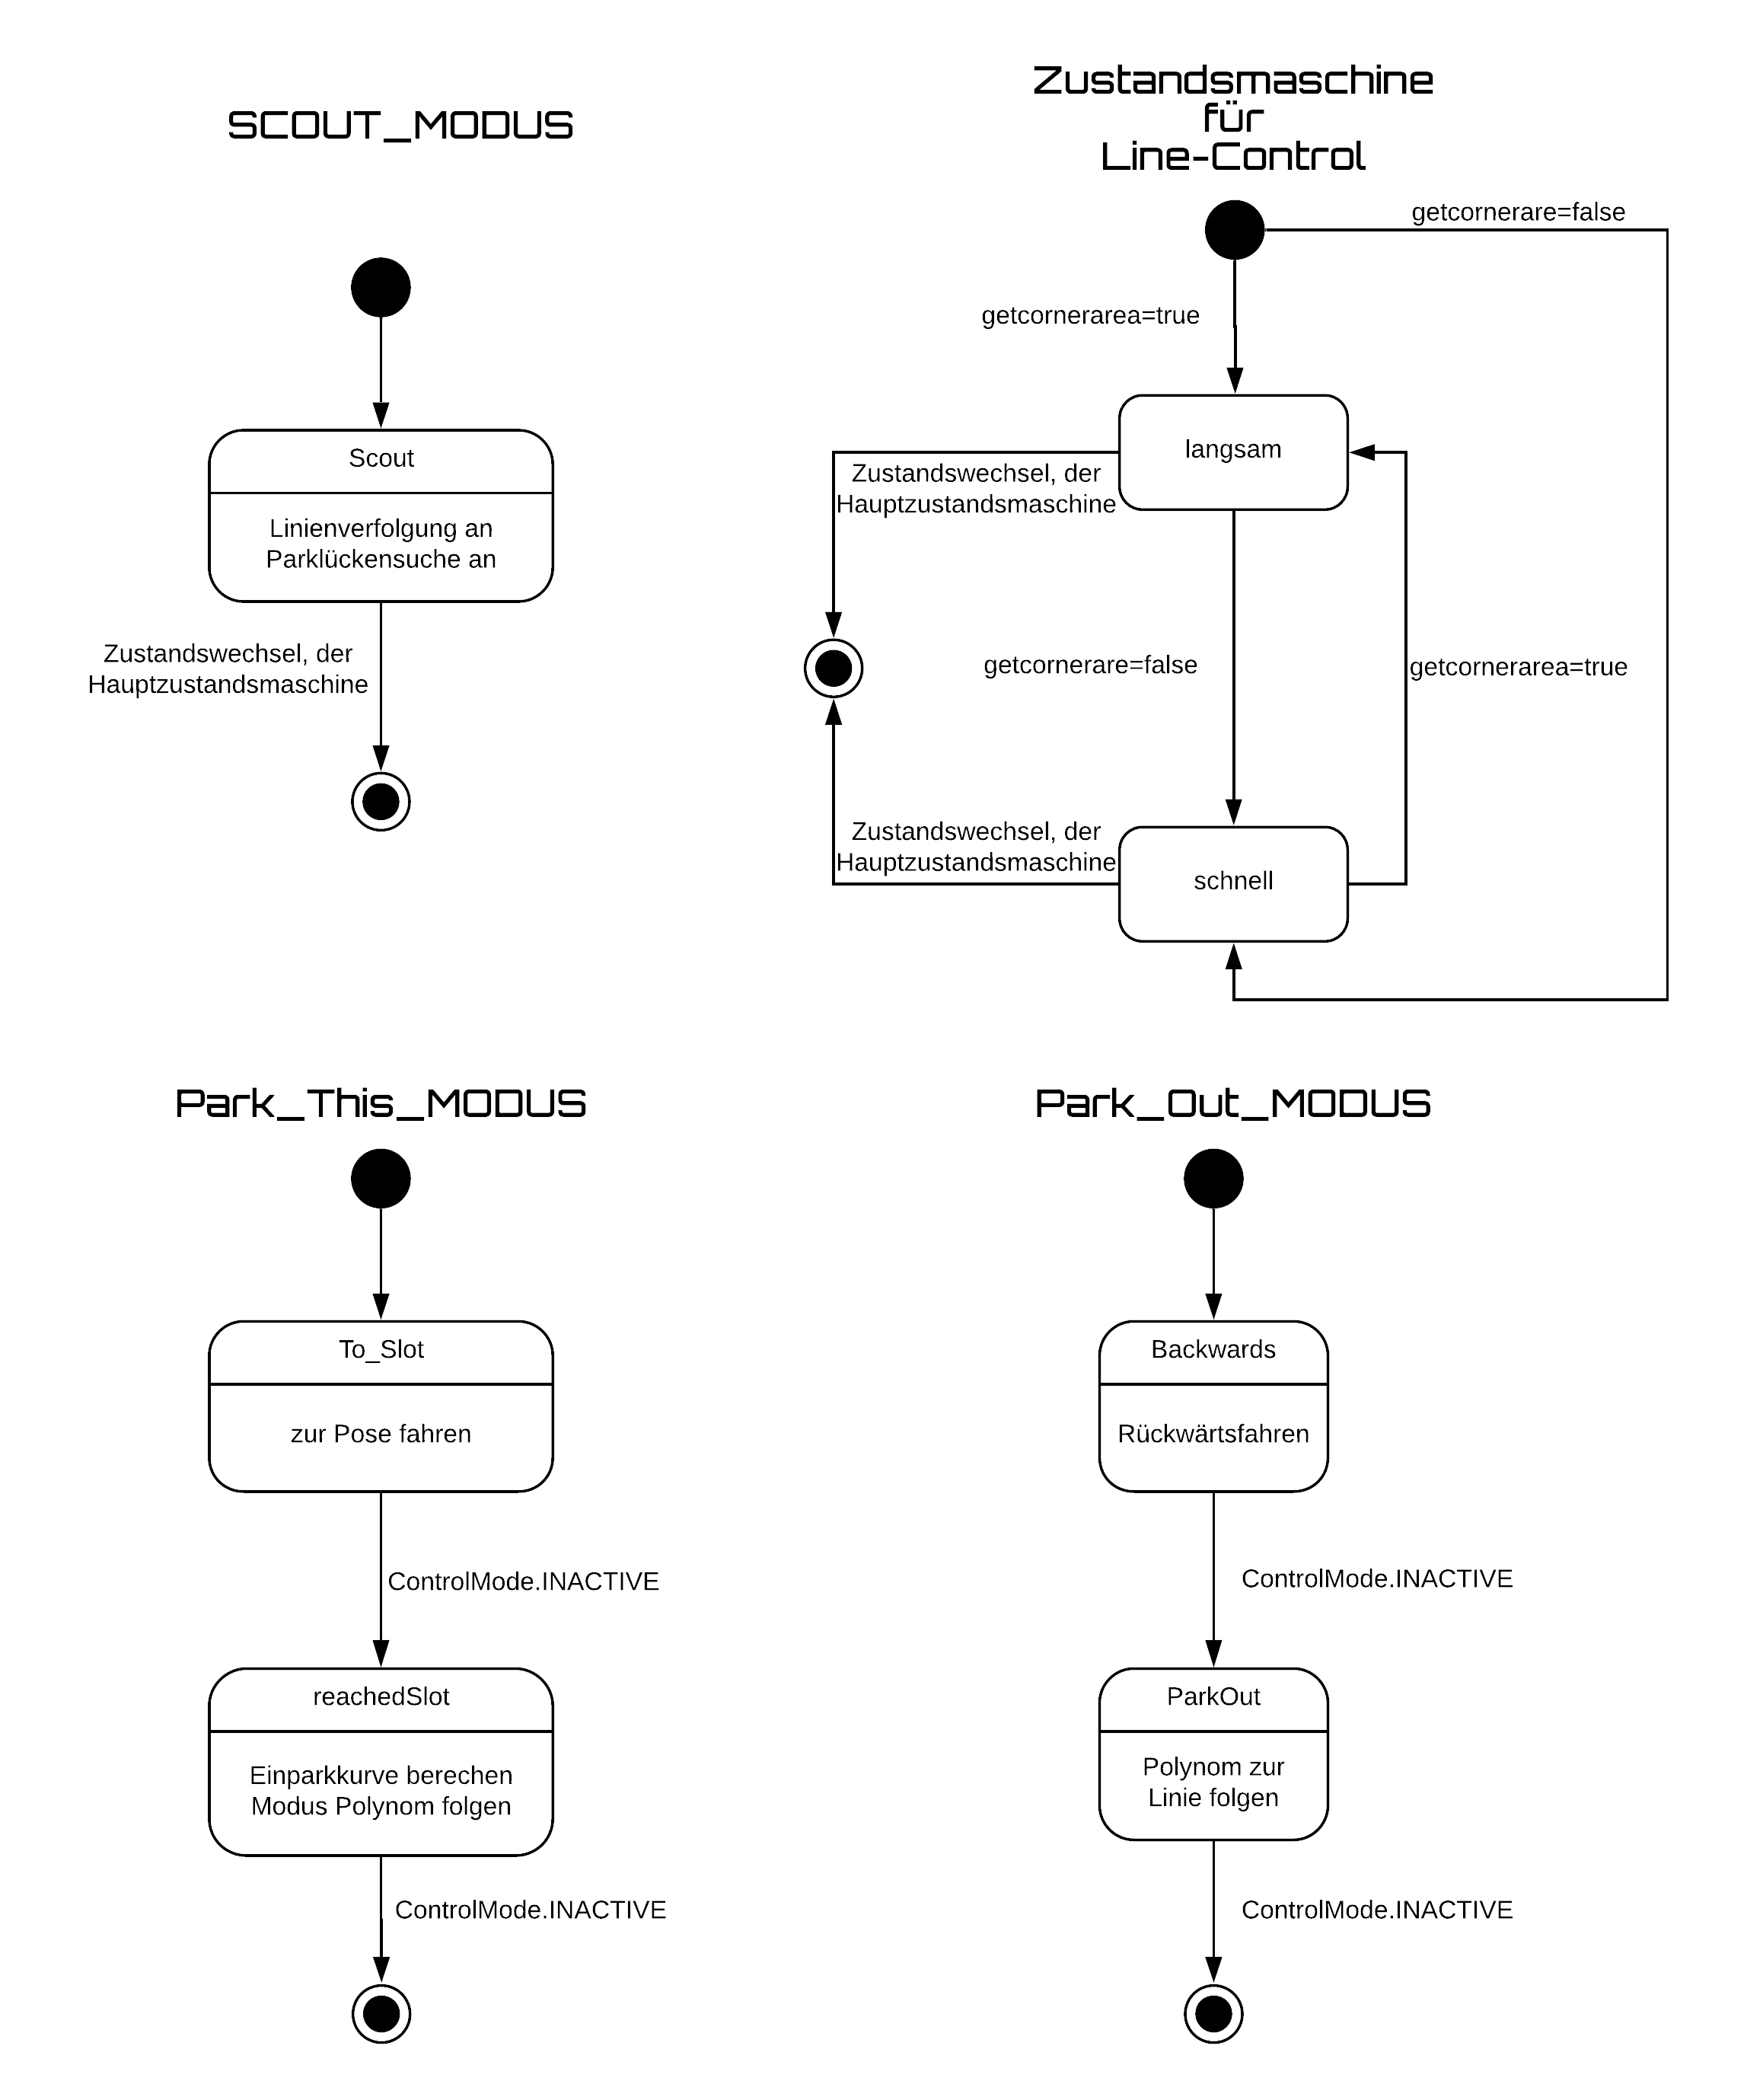
\includegraphics[width=0.9\textwidth]{Subzustandsmaschine}
	\caption{Entwurf Unterzustandsmaschine}
	\label{img:grafik-Unterzustandsautomat}
\end{figure}
